\documentclass[twocolumn]{article}
\author{}
\usepackage{graphicx} %I need to include some graphs in this document
\usepackage{amsmath}
\usepackage{caption}
\usepackage{subcaption}
%\usepackage[margin=1.4in]{geometry}
\begin{document}
In our calculations, the standard deviation of temperature in a certain slab $m$ is expressed as
\begin{equation}
\sigma_{m,s}=\sqrt{\frac{\sum\limits_{i=1}^\mathcal{N}\left( T_{m,i}-\overline{T}_m\right)}{\mathcal{N}-1}}
\end{equation}
where $\overline{T}_m$ is the average value for measurements $T_{m,i}$ and $\mathcal{N}$ represents the total number of measurements.The standard deviation of the averaged value $\overline{T}_m$, therefore, is given by
\begin{align}
\sigma_m &=\frac{\sigma_{m,s}}{\sqrt{\mathcal{N}}}\\
&=\sqrt{\frac{\sum\limits_{i=1}^\mathcal{N}\left( T_{m,i}-\overline{T}_m\right)}{\mathcal{N}(\mathcal{N}-1)}}
\end{align}
\paragraph*{}
With a set of data $(\overline{T}_m,\sigma_m)$ where $m$ goes from 0 to N-1 in our model, we do the fit to the cosine function to determine and fitting parameter of amplitude, which is $\Delta T$ in Eq.(1). The standard deviation of $\Delta T$ is determined at the same time.Then by using Eq.(2) we can get a relation between $\sigma_{\Delta T}$ and $\sigma_{\kappa_{\mbox{eff}}}$, which is
\begin{equation}
\frac{\sigma_{\kappa}}{\kappa_{\mbox{eff}}}=\frac{\sigma_{\Delta T}}{\Delta T}
\end{equation}
Thus $\sigma_{\kappa_{\mbox{eff}}}=\kappa_{\mbox{eff}}\sigma_{\Delta{T}}/\Delta{T}$ gives the standard deviation of $\kappa$.
\setcounter{section}{2}
\begin{center}
\section{TEST ON LIQUID}
\end{center}
\setcounter{equation}{9}
\subsection*{COMPUTATION DETAILS}
\paragraph*{}
The system we are using consists of 2592 Lennard-Jones atoms in an orthorbombic supercell which is of size $10.059\sigma\times10.059\sigma\times30.176\sigma$ in reduced unit, with the number density $\rho^*=0.849$. Periodical boundary condition is used and our supercell is divided into 20 slabs (0-19). A time step $\Delta t^*=6.965\times10^{-3}$ is used and the cut off distance for the Lennard-Jones potential is $3\sigma$. We tested on heat imposes with different amplitudes while imposing the heat input at the same step interval of 60. All systems are running with constant total energy with an average temperature close to $T^*=0.70$.
\paragraph*{}
We tested on four different heat inputs. The resulting temperature profiles are shown in Fig.1. All inputs are imposed every 60 time steps, which we believe will not affect the results too much. The flux is imposed between pair slabs centering slab 4 and slab 14 respectively, namely slab 0 and slab 8, slab 9 and slab 19 etc. Slab 0-3 and 15-19 are set to be cold slabs while slabs numbering 5-8 and 9-13 are hot slabs in this case. We take an impose of the form $\dot{e}(m)=-\dot{e}cos(m/20)$, which is to say, the heat inputs for slab 0-19, on average, are $-\dot{e}cos(\pi/20)$,$-\dot{e}cos(2\pi/10)$,$-\dot{e}cos(3\pi/20)$ etc. Then measurements on the slab temperature are conducted. We do the fitting to obtain the value of $\Delta T$ by fitting the data with cosine function $-\Delta Tcos(m/20)$ and calculating $\kappa$ with equation below:
\begin{equation}
\kappa_{\mbox{eff}}(N)=\frac{\dot{e}/\Delta T}{4\sin^2(\pi/20)}\times\frac{A}{\sigma}
\end{equation}
with the fact that in the case of liquid $\kappa=\kappa_{\mbox{eff}}(N)$.
\subsection*{RESULTS AND DISCUSSION}

\begin{figure}[h] % [h]make the graph in the current location
\centering
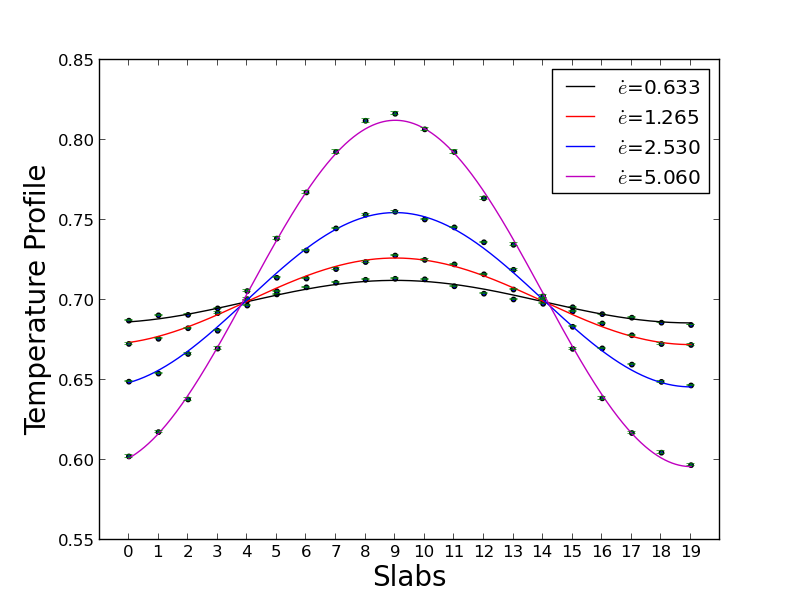
\includegraphics[width=\linewidth]{Experiments.png}
\caption{Temperature Profile}
\end{figure}
\paragraph*{}
The variation in temperature increases with the amplitude of the heat input and the speed of convergence turns out to increase with $\dot{e}$ as well. The results are summarized in Table 1 and all calculated values are companied by an relative error within 4\%. The experiment data of liquid Argon is given under $T^*=0.71$ with the number of density $\rho^*=0.84$, serving as a reference of our calculation.   
\begin{table}[ht]
\centering
\caption{Thermal conductivity for L-J liquid at T=0.69 and $\rho=0.85$}

\begin{tabular}{p{1.6cm}|p{1.7cm} p{1.7cm} p{1.7cm}}
\hline
\hline
{$\dot{e}$}&{$\kappa(\sigma_\kappa)$ }&{$\sigma_\kappa/\kappa$}&{Stimulation Steps}\\
\hline*
0.633                              &   7.25(0.24)   & 3.26\%         & 576210\\
1.265                              &   7.12(0.12)   & 1.69\%         & 96000\\
1.265                              &   7.00(0.07)   & 1.03\%         & 192010\\
2.530                              &   6.81(0.08)   & 1.17\%         & 96000\\
5.060                              &   7.12(0.05)   & 0.70\%        & 24000\\
\hline
Experiment                         &   7.02\footnote{Experiment data for Argon    Handbook of Chemistry and Physics, 74th ed., edited by D. R. Lide Chemical Rubber, Boca Raton, 1993} \\
\hline
\end{tabular}
\end{table}
\paragraph*{}
It is worth to notice that step interval is chosen to be $W=60$ in our test. Firstly, in order to ensure the effectiveness of the of this algorithm the result of $X$ in Eqs.(7) is supposed to be greater than 1. While Eqs.(4) can be written as

\begin{equation}
%\centering
X = [\delta-(v_H^2-v_C^2)]\cdot\frac{\delta}{\lvert \vec{v}_H+\vec{v}_C\lvert^2}\cdot\frac{1}{b^2r^2-(\vec{b}\cdot\vec{r})^2}
\end{equation}
\paragraph*{}
For safety in evolutions, we'd better keep $X$ negative. As shown in Eqs.(10) the last two terms are positive so $\delta-(v_H^2-v_C^2)=2\Delta/m-(v_H^2-v_C^2)$ dominates. It is found in tests that $v_H^2-v_C^2$ sometimes touches the ground of 3(in L-J reduced units), so if $W$ were set to be 480 in this case, for instance, we would soon find errors in the data. One may insist on a $W$ which is much smaller than 60 to enable inputs with larger amplitudes for the simple reason that large imposes converge much faster. However, this proves unnecessary: it has been shown in Muller-Plathe's method that validity of linear response theory breaks down for large variation with $W=15$, which is parallel to the impose with  $\dot{e}=10.120$ in our theory. So even if, with lower $W$ and larger input amplitude, there is nothing wrong with the calculation of vector $\vec{w}$, it is meaningless to do calculations of this kind without the validity of linear response theory. It is been tested that $W=60$ does not work for $\dot{e}=10.120$, therefore, our choice of $W$ seems quite reasonable. Secondly, in spite of the fact lowing the $W$ will not considerably affect the results, doing the impose too frequently might disturb the fitting since the system is not stable all the time, which as a result, influences the convergence of error.
\paragraph*{}
Comparing this new algorithm with the direct method proposed by Muller-Plathe, we used the same heat input as reference 3 on the system we are testing above. It is reasonable to evolve two systems with the same temperature variation, which means the maximum difference in slab temperatures should be the same and in order to do this, we test Muller-Plathe's method with exchange step $W=120$. The results below also come from a same equilibrium input-they start from a same equilibrium state of the supercell system.
\begin{figure}[h]
\centering
  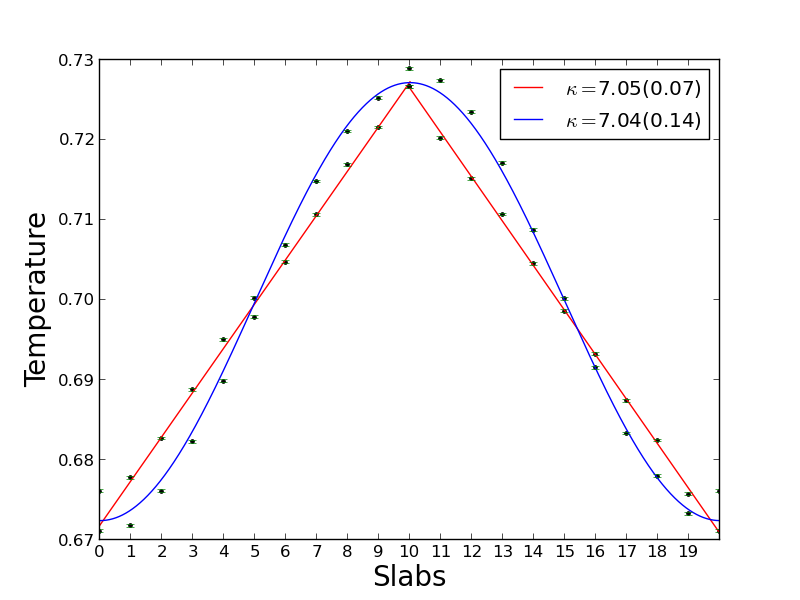
\includegraphics[width=\linewidth]{amplitude.png}
\caption{Comparison Under Same Temperature Variation}
\end{figure}
\subsubsection*{}
\paragraph*{}
The evolution of relative error of $\kappa$ is shown in Fig.3 and there are several characteristics here. Firstly, it seems apparent that Muller-Plathe's method converges faster at the beginning of the evolution but as time goes by, the relative error of $\kappa$ drops off more quickly by exploiting the slabs for the heat input and as a result, the relative error of the new algorithm falls below the original one. A second thing to notice is that the new algorithm is removing error more smoothly whereas the errors with red line (orignal direct method) tends to fluctuate while descending.
\begin{figure}[h] % [h]make the graph in the current location
\centering
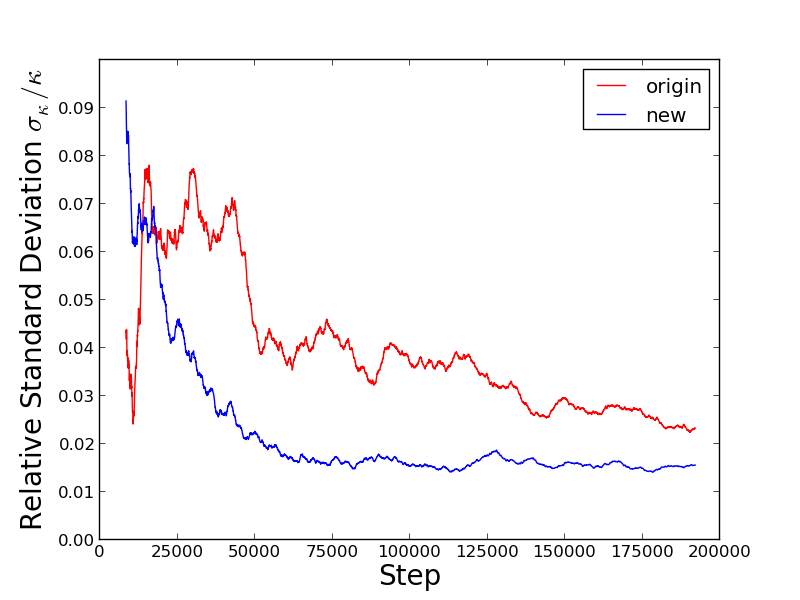
\includegraphics[width=\linewidth]{RelativeError.png}
\caption{Evolution of Relative Error}
\end{figure}
\paragraph*{}
In order to further compare the two algorithms, we now look at the ratio of time step for the algorithms to reach certain accuracy. Here, we define the moment for an algorithm to give certain accuracy as the instant, during the stimulation, at which the relative error of $\kappa$ the algorithm predicts falls below certain number. This may not be a very convincing definition. However, if we look at the ratio of time steps for different relative errors,a snapshot for data in this process will tell us how they are behaving on average.
\paragraph*{}
Fig.4 gives the ratio of the time steps for different accuracies. The ratio is defined as the time step the  new algorithm requires over the old one. Anyone would predict that the ratio will settle down at the point (0,1) with the simple fact that none of these algorithms can possibly gives an accuracy of zero. So if we run the system long enough, we will get a curve that end up at (0,1) but it must be very time-consuming: we have run our programs for nearly two days and the two algorithms give an accuracy of around 2\%. Furthermore, this curve seems to be a concave one for the behaviour presented. This concave curve tells us that the new algorithm can not only converge faster but give higher accuracy as well.
\begin{figure}[h] % [h]make the graph in the current location
\centering
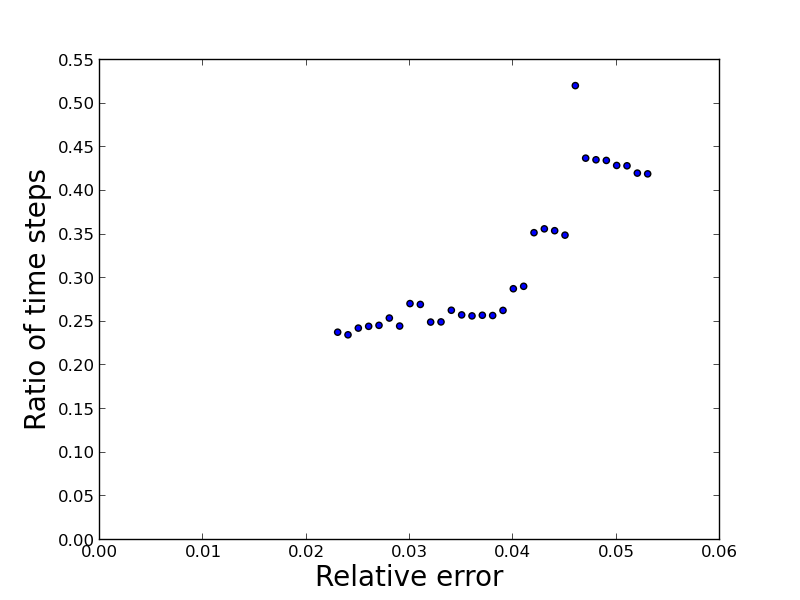
\includegraphics[width=\linewidth]{Comparison.png}
\caption{Ratio of Time Steps}
\end{figure}
\end{document}